%%%%%%%%%%%%%%%%%%%%%%%%%%%%%%%%%%%%%%%%%
% Lachaise Assignment
% LaTeX Template
% Version 1.0 (26/6/2018)
%
% This template originates from:
% http://www.LaTeXTemplates.com
%
% Authors:
% Marion Lachaise & François Févotte
% Vel (vel@LaTeXTemplates.com)
%
% License:
% CC BY-NC-SA 3.0 (http://creativecommons.org/licenses/by-nc-sa/3.0/)
% 
%%%%%%%%%%%%%%%%%%%%%%%%%%%%%%%%%%%%%%%%%

%----------------------------------------------------------------------------------------
%	PACKAGES AND OTHER DOCUMENT CONFIGURATIONS
%----------------------------------------------------------------------------------------


%Bibliograpy

\documentclass{article}

%%%%%%%%%%%%%%%%%%%%%%%%%%%%%%%%%%%%%%%%%
% Lachaise Assignment
% Structure Specification File
% Version 1.0 (26/6/2018)
%
% This template originates from:
% http://www.LaTeXTemplates.com
%
% Authors:
% Marion Lachaise & François Févotte
% Vel (vel@LaTeXTemplates.com)
%
% License:
% CC BY-NC-SA 3.0 (http://creativecommons.org/licenses/by-nc-sa/3.0/)
% 
%%%%%%%%%%%%%%%%%%%%%%%%%%%%%%%%%%%%%%%%%

%----------------------------------------------------------------------------------------
%	PACKAGES AND OTHER DOCUMENT CONFIGURATIONS
%----------------------------------------------------------------------------------------

\usepackage{amsmath,amsfonts,stmaryrd,amssymb} % Math packages

\usepackage{enumerate} % Custom item numbers for enumerations

\usepackage[ruled]{algorithm2e} % Algorithms

\usepackage[framemethod=tikz]{mdframed} % Allows defining custom boxed/framed environments

\usepackage{listings} % File listings, with syntax highlighting
\lstset{
	basicstyle=\ttfamily, % Typeset listings in monospace font
}


%Spanish languaje 
\usepackage[spanish]{babel}
%Bibliograpy
\usepackage{cite}
%Paragraph Space
\setlength{\parskip}{1em}
%Float
\usepackage{float}

% Footer and header styles 
\usepackage{fancyhdr}
\thispagestyle{plain}
%\pagestyle{fancy}
%\fancyhf{}
%\fancyhead[LE,RO]{Tarea 3}
%\fancyhead[RE,LO]{\leftmark}
%\fancyfoot[CE,CO]{\thepage }
%\fancyfoot[LE,RO]{
%	\begin{figure}[H]
%		\flushright
%		\includegraphics[width=4cm, height=2cm]{./img/tec.png}
%	\end{figure}
%}

\renewcommand{\baselinestretch}{1.5}

%----------------------------------------------------------------------------------------
%	DOCUMENT MARGINS
%----------------------------------------------------------------------------------------

\usepackage{geometry} % Required for adjusting page dimensions and margins

\geometry{
	paper=a4paper, % Paper size, change to letterpaper for US letter size
	top=2.5cm, % Top margin
	bottom=3cm, % Bottom margin
	left=2.5cm, % Left margin
	right=2.5cm, % Right margin
	headheight=14pt, % Header height
	footskip=1.5cm, % Space from the bottom margin to the baseline of the footer
	headsep=1.2cm, % Space from the top margin to the baseline of the header
	%showframe, % Uncomment to show how the type block is set on the page
}

%----------------------------------------------------------------------------------------
%	FONTS
%----------------------------------------------------------------------------------------

\usepackage[utf8]{inputenc} % Required for inputting international characters
\usepackage[T1]{fontenc} % Output font encoding for international characters

\usepackage{XCharter} % Use the XCharter fonts

%----------------------------------------------------------------------------------------
%	COMMAND LINE ENVIRONMENT
%----------------------------------------------------------------------------------------

% Usage:
% \begin{commandline}
%	\begin{verbatim}
%		$ ls
%		
%		Applications	Desktop	...
%	\end{verbatim}
% \end{commandline}

\mdfdefinestyle{commandline}{
	leftmargin=10pt,
	rightmargin=10pt,
	innerleftmargin=15pt,
	middlelinecolor=black!50!white,
	middlelinewidth=2pt,
	frametitlerule=false,
	backgroundcolor=black!5!white,
	frametitle={Command Line},
	frametitlefont={\normalfont\sffamily\color{white}\hspace{-1em}},
	frametitlebackgroundcolor=black!50!white,
	nobreak,
}

% Define a custom environment for command-line snapshots
\newenvironment{commandline}{
	\medskip
	\begin{mdframed}[style=commandline]
}{
	\end{mdframed}
	\medskip
}

%----------------------------------------------------------------------------------------
%	FILE CONTENTS ENVIRONMENT
%----------------------------------------------------------------------------------------

% Usage:
% \begin{file}[optional filename, defaults to "File"]
%	File contents, for example, with a listings environment
% \end{file}

\mdfdefinestyle{file}{
	innertopmargin=1.6\baselineskip,
	innerbottommargin=0.8\baselineskip,
	topline=false, bottomline=false,
	leftline=false, rightline=false,
	leftmargin=2cm,
	rightmargin=2cm,
	singleextra={%
		\draw[fill=black!10!white](P)++(0,-1.2em)rectangle(P-|O);
		\node[anchor=north west]
		at(P-|O){\ttfamily\mdfilename};
		%
		\def\l{3em}
		\draw(O-|P)++(-\l,0)--++(\l,\l)--(P)--(P-|O)--(O)--cycle;
		\draw(O-|P)++(-\l,0)--++(0,\l)--++(\l,0);
	},
	nobreak,
}

% Define a custom environment for file contents
\newenvironment{file}[1][File]{ % Set the default filename to "File"
	\medskip
	\newcommand{\mdfilename}{#1}
	\begin{mdframed}[style=file]
}{
	\end{mdframed}
	\medskip
}

%----------------------------------------------------------------------------------------
%	NUMBERED QUESTIONS ENVIRONMENT
%----------------------------------------------------------------------------------------

% Usage:
% \begin{question}[optional title]
%	Question contents
% \end{question}

\mdfdefinestyle{question}{
	innertopmargin=1.2\baselineskip,
	innerbottommargin=0.8\baselineskip,
	roundcorner=5pt,
	nobreak,
	singleextra={%
		\draw(P-|O)node[xshift=1em,anchor=west,fill=white,draw,rounded corners=5pt]{%
		Question \theQuestion\questionTitle};
	},
}

\newcounter{Question} % Stores the current question number that gets iterated with each new question

% Define a custom environment for numbered questions
\newenvironment{question}[1][\unskip]{
	\bigskip
	\stepcounter{Question}
	\newcommand{\questionTitle}{~#1}
	\begin{mdframed}[style=question]
}{
	\end{mdframed}
	\medskip
}

%----------------------------------------------------------------------------------------
%	WARNING TEXT ENVIRONMENT
%----------------------------------------------------------------------------------------

% Usage:
% \begin{warn}[optional title, defaults to "Warning:"]
%	Contents
% \end{warn}

\mdfdefinestyle{warning}{
	topline=false, bottomline=false,
	leftline=false, rightline=false,
	nobreak,
	singleextra={%
		\draw(P-|O)++(-0.5em,0)node(tmp1){};
		\draw(P-|O)++(0.5em,0)node(tmp2){};
		\fill[black,rotate around={45:(P-|O)}](tmp1)rectangle(tmp2);
		\node at(P-|O){\color{white}\scriptsize\bf !};
		\draw[very thick](P-|O)++(0,-1em)--(O);%--(O-|P);
	}
}

% Define a custom environment for warning text
\newenvironment{warn}[1][Warning:]{ % Set the default warning to "Warning:"
	\medskip
	\begin{mdframed}[style=warning]
		\noindent{\textbf{#1}}
}{
	\end{mdframed}
}

%----------------------------------------------------------------------------------------
%	INFORMATION ENVIRONMENT
%----------------------------------------------------------------------------------------

% Usage:
% \begin{info}[optional title, defaults to "Info:"]
% 	contents
% 	\end{info}

\mdfdefinestyle{info}{%
	topline=false, bottomline=false,
	leftline=false, rightline=false,
	nobreak,
	singleextra={%
		\fill[black](P-|O)circle[radius=0.4em];
		\node at(P-|O){\color{white}\scriptsize\bf i};
		\draw[very thick](P-|O)++(0,-0.8em)--(O);%--(O-|P);
	}
}

% Define a custom environment for information
\newenvironment{info}[1][Info:]{ % Set the default title to "Info:"
	\medskip
	\begin{mdframed}[style=info]
		\noindent{\textbf{#1}}
}{
	\end{mdframed}
}

 % Include the file specifying the document structure and custom commands


%----------------------------------------------------------------------------------------
%	ASSIGNMENT INFORMATION
%----------------------------------------------------------------------------------------

\title{Proyecto: Crecimiento económico y su relación con energías limpias en la región latinoamericana
} % Title of the assignment

\author{Geykel Hodgson Chavaría\\ 
Aaron Sibaja Villalobos  
} % Author name and email address

\date{Instituto  Tecnológico de Costa Rica -- \today} % University, school and/or department name(s) and a date

%----------------------------------------------------------------------------------------

\begin{document}

%Rename table name
\renewcommand{\listtablename}{Índice de tablas}
\renewcommand{\tablename}{Tabla} 

\maketitle % Print the title

%----------------------------------------------------------------------------------------
%	INTRODUCTION
%----------------------------------------------------------------------------------------

\section{Definición de problema}
Se sabe que existe una relación entre el consumo eléctrico y el crecimiento económico de un país, lo que no esta claro es si las energías limpias influyen de alguna forma en el crecimiento del PIB. El propósito de esta visualización es identificar las relaciones en el crecimiento económico al comparar países que apuesta por energía renovables contra los que utilizan derribados del petroleo en América Latina.

\section{Objetivos}
\subsection{General}
Identificar las relaciones del crecimiento económico y el uso de energías limpias en América Latina.
\subsection{Específicos }
\begin{itemize}
    \item Identificar los tipos de energía más usados en América Latina.
    % \item Determinar el crecimiento del PIB de los países de América Latina.
    \item Conocer la cobertura de acceso a la electricidad por país en América Latina.
    \item Comparar crecimiento económico entre países que apuestan por energías limpias contra países que utilizan combustibles fósiles en América Latina.
    \item Evidenciar causalidad entre el consumo de fuentes renovables y el incremento del PIB.
\end{itemize}

\section{Contexto}




La electricidad corresponde a un pilar fundamental para progreso de una nación.   Existe un cantidad significante de textos y artículos que han demostrado cómo el crecimiento  de la actividad económica de un país se encuentra relacionado con el uso de la electricidad. Esto evidencia un crecimiento en la población y en la generación de bienes y servicios \cite{chen_relationship_2007}. 

El PIB  corresponde a la suma del sector  industrial, agricultura y de servicios de un país, en otras palabras, el valor en el mercado de sus productos y servicios. El sector agricultura y de servicios son sectores poco dependientes de la electricidad sin embargo el sector industrial si depende mayormente de la electricidad. Esto da cómo que la relación entre el PIB y el consumo de electricidad en países que basan mayormente su economía en el sector industrial. Para el 2017, 20$\%$ del PIB en Estados Unidos estaba conformada por el sector industrial \cite{noauthor_why_2014}. 

Algunos países que pertenecen al OCDE (Organización para la Cooperación y el Desarrollo Económicos ) cómo por ejemplo: Canadá, Reino Unido, Suiza, USA, Alemania y Colombia tienen economías fuertemente influenciadas por  la manufactura, sin embargo continuamente se actualizan a tecnologías que hacen uso de un menor recurso eléctrico y son más eficientes \cite{noauthor_link_nodate}. Los paises que no forman parte del OCDE cómo China, India y Brazil, presentan economías en crecimiento generalmente basadas en sector manufactura. Estas economías en particular presentan tecnologías más antiguas que requieren un mayor consumo de energía para poder generar bienes. En el 2011 el total de uso de energía de los países que no pertenecen al OCDE sobrepasó a los miembros del OCDE. Esto evidencia que probablemente la mayor cantidad de consumo eléctrico en el futuro va a concentrar en los paises que no forman parte del OCDE y el camino que elijan para sus respectivas economías. 










\section{Metodología }
Para la realización de este trabajo se decidió utilizar la metodología propuesta por Benjamín Fry \cite{fry2008visualizing}, este método consta de siete etapas:
\begin{itemize}
    \item \textbf{Recolectar datos: } 
    esta etapa consiste en buscar y obtener el conjunto de datos que vamos a utilizar, lo principal es conseguir fuentes de datos confiables, provenientes de otros estudios académicos o algún organismo oficial. En esta fase también se define como los datos recolectados van a ser accedidos por los usuarios.
    \item \textbf{Estructuración de los datos: } 
    una vez que se tienen datos confiables, hay que ordenarlos y categorizarlos para que estos adquieran una estructura bien definida. Si lo datos no están estructurados correctamente se dificulta el análisis y la visualización de los mismos.
    \item \textbf{Filtrar: }
    en este paso se debe decidir desde el punto de vista de la visualización cuales datos son útiles y aportan información relevante. Los datos que no se consideren relevantes son filtrados y no se toman en cuenta para la representación.
    \item \textbf{Extraer: }
    se procede a convertir, los datos relevantes, en variables que denoten los valores o cantidades que necesitamos analizar y mostrar a través de la visualización. Esto se logra al aplicar métodos estadísticos o de minería de datos que permitan colocar los datos en un contexto matemático.
    \item \textbf{Representar:}
    se escoge un modelo visual básico (Gráfico de barras, arboles, listas, entre otros), apropiado para una visualización clara y concisa de las variables creadas en el paso anterior.
    \item \textbf{Refinar: }
    trabajar de forma iterativa sobre el modelo visual básico con el fin de mejorarlo y que sea capaz de transmitir la información de forma clara, además debe ser atractivo y cautivador para el usuario.  
    \item \textbf{Interactuar: }
    agregar elementos que permitan al usuario la manipulación y el control de las características que son visibles. Los usuarios deben poder seleccionar diferentes rangos de datos e intervalos de tiempo que le permitan analizar la información presentada desde múltiples puntos de vista.  
\end{itemize}

\section{Alcance Esperado}

El propósito principal de la visualización es permitir el análisis de la relación que existe entre el crecimiento económico y el consumo de energías. El crecimiento económicos de un país se medirá en base al PIB y las energías que se presentaran serán de dos tipos: las renovables y las derivadas del petroleo. La visualización presentara los datos de los países de América Latina en un periodo de 15 años que van desde 2000 hasta el 2015. También se incluirá el porcentaje de cobertura eléctrica de cada país.

%*** Exploratorio
%- Examinar un tema poco estudiado (se ha estudiado mucho la relación entre electricidad y crecimiento económico pero poco o nada en relación al tipo de energía utilizado)
%- Indaga desde una perspectiva innovadora (la perspectiva de energías renovables o limpias)
%- Ayuda a identificar conceptos promisorios (Identificar causalidad en el uso de energías limpias y crecimiento económico)
%
%-Prepara el terreno para nuevos estudios, que otros estudios podrían derivarse?
%
%el crecimiento economico se va medir desde el punto de vista del PIB.
%se dividen los tipos de energia entre derivados del petroleo y energias renovables (cuales energias renovables toma encuenta el banco mundial?)
%muestra el porcentaje de acceso a la electricidad en cada pais ? %puede no ser relevante 

% Please add the following required packages to your document preamble:
% \usepackage{multirow}
\begin{table}[H]
\centering
\caption{Países incluidos en la visualización }
\begin{tabular}{|l|l|}
\hline
\textbf{Región}                 & \textbf{País} \\ \hline
Sudamérica   & Argentina     \\ \cline{2-2} 
                                & Bolivia       \\ \cline{2-2} 
                                & Brasil        \\ \cline{2-2} 
                                & Chile         \\ \cline{2-2} 
                                & Colombia      \\ \cline{2-2} 
                                & Ecuador       \\ \cline{2-2} 
                                & Paraguay      \\ \cline{2-2} 
                                & Perú          \\ \cline{2-2} 
                                & Uruguay       \\ \cline{2-2} 
                                & Venezuela     \\ \hline
Centro América & Costa Rica    \\ \cline{2-2} 
                                & El Salvador   \\ \cline{2-2} 
                                & Guatemala     \\ \cline{2-2} 
                                & Honduras      \\ \cline{2-2} 
                                & Nicaragua     \\ \cline{2-2} 
                                & Panamá        \\ \hline
Norte América                   & México        \\ \hline
\end{tabular}
\end{table}

\section{Recursos requeridos}

Se va a utilizar los datos recolectados por el banco mundial los cuales son presentados mediante su página web oficial \cite{noauthor_indicadores_nodate}. Este portal contiene 76 base de datos en total, las cuales abarcan 264 países. Cada base de datos está compuesta por series, en la base de datos principal \textit{indicadores del desarrollo mundial} se pueden encontrar 1429, las series corresponden a indicadores y se encuentran etiquetadas con su respectiva descripción y con diferente medición numérica.

La página web permite realizar filtros de forma que se puedan tener varias regiones del globo. Además admite seleccionar el tiempo en los datos de forma que cada indicador es anual para cada país estos se encuentran desde 1966 hasta el 2019. 

Es posible extraer los datos en formato de Excel, CSV o en TSV. La descarga es un archivo comprimido que contiene dos archivos, uno con la data con el formato seleccionado y otro  archivo con metadata detallada sobre cada uno de los indicadores cómo por ejemplo: fuente, descripción larga y corta, licencia y periodicidad. 


\section{Lista de riesgos y estrategias de mitigación}
\begin{enumerate}
    \item Poca experiencia en el uso de herramientas y diseño de visualizaciones.
    \begin{itemize}
        \item Avance limitado en la creación de la visualización.
        \item Demoras en los entregables.
        \item Aumenta la dificultad del desarrollo.
        \item Visualizaciones poco atractivas.
        \item Carencia de interactividad.
    \end{itemize}
    
\textbf{Mitigación:}
  \begin{itemize}
      \item Buscar herramientas afines a los lenguajes de programación conocidos.
      \item Buscar una herramienta con amplio soporte y documentación.
      \item Seleccionar la herramienta en las primeras etapas, con el fin de tener tiempo para aprender a utilizarla.
      \item Buscar y estudiar ejemplos de visualizaciones con elementos en común.
  \end{itemize}

    
    
\item Falta de información en la base de datos del Banco Mundial para los países elegidos.
    \begin{itemize}
        \item  No poder cumplir con el alcance propuesto.
        \item Limita la comparación entre países.
    \end{itemize}
   

\textbf{Mitigación:}

\begin{itemize}
    \item Buscar otras fuentes de datos.
    \item Reducir la lista de países.
    \item Reducir o cambiar el periodo del estudio. 
\end{itemize}
  
    
\item Poca documentación sobre la estructura de los datos.
\begin{itemize}
    \item Puede producir malas interpretaciones en los datos.
    \item Aumenta la dificultad del desarrollo.
    \item Demoras en los entregables.
    \item Conlleva a resultados erróneos.
\end{itemize}
    
\textbf{Mitigación:}
\begin{itemize}
    \item Buscar fuentes confiables y reconocidas.
    \item Preferir fuentes con metadata.
\end{itemize}


\newpage 

\item Alcance muy amplio.
\begin{itemize}
    \item Demoras en los entregables.
    \item Falta de tiempo para completar las visualizaciones.
    \item Poca representación de los datos.
    \item Poca claridad en las relaciones.
\end{itemize}
   
    
\textbf{Mitigación:}
    \begin{itemize}
        \item Cumplir con el cronograma.
        \item Dividir el trabajo de forma eficiente y clara.
        \item Reunirse periódicamente para mostrar avances y planear la siguiente etapa.
    \end{itemize}
    
\end{enumerate}


%The below command generates a 4 X 5 risk matrix with ALARP regions for initial risk matrix.

% Please add the following required packages to your document preamble:
% \usepackage[table,xcdraw]{xcolor}
% If you use beamer only pass "xcolor=table" option, i.e. \documentclass[xcolor=table]{beamer}
% Please add the following required packages to your document preamble:
% \usepackage[table,xcdraw]{xcolor}
% If you use beamer only pass "xcolor=table" option, i.e. \documentclass[xcolor=table]{beamer}
\begin{table}[H]
\centering
\caption{Matriz de riesgos}
\begin{tabular}{|l|l|l|l|l|l|}
\hline
                      & \multicolumn{5}{c|}{\textbf{Consecuencia}}                                                                                                                  \\ \hline
\textbf{Probabilidad} & \textbf{Muy Bajo}        & \textbf{Bajo}            & \textbf{Moderado}        & \textbf{Alto}            & \textbf{Muy Alto}                               \\ \hline
\textbf{Muy Alto}     & \cellcolor{yellow! 50}& \cellcolor{yellow! 50}& \cellcolor{yellow! 50}& \cellcolor{red! 50}  & \cellcolor{red! 50}  \\ \hline
\textbf{Alto}         & \cellcolor{yellow! 50}& \cellcolor{yellow! 50}& \cellcolor{yellow! 50}& \cellcolor{red! 50}  & \cellcolor{red! 50}  \\ \hline
\textbf{Moderado}     & \cellcolor{green! 50}  & \cellcolor{yellow! 50}& \cellcolor{yellow! 50}4 & \cellcolor{yellow! 50}& \cellcolor{red! 50}  1 \\ \hline
\textbf{Bajo}         & \cellcolor{green! 50}  & \cellcolor{green! 50}  & \cellcolor{yellow! 50}  & \cellcolor{yellow! 50} 2 ,3 & \cellcolor{red! 50}  \\ \hline
\textbf{Muy Bajo}     & \cellcolor{green! 50}  & \cellcolor{green! 50}  & \cellcolor{yellow! 50}& \cellcolor{yellow! 50}& \cellcolor{yellow! 50}\\ \hline
\end{tabular}
\end{table}


%The command below provides the legend for the Risk Matrix

\begin{table}[H]
\centering
%\scriptsize
\caption{Legenda de color de la matriz de riesgo}
\begin{tabular}{|p{2cm}|p{10cm}|}
\hline \bf Color & \bf Legenda \\
\hline \cellcolor{red! 50} & Aceptable - Se requiere reducción de riesgo\\ [10pt]
\hline \cellcolor{yellow! 50} & Aceptable - Considere reducir el riesgo. \\[10pt]
\hline \cellcolor{green! 50} & Aceptable \\ [10pt]
\hline
\end{tabular}
\end{table}


\section{Cronograma}

\begin{figure}[H]
		\centering
		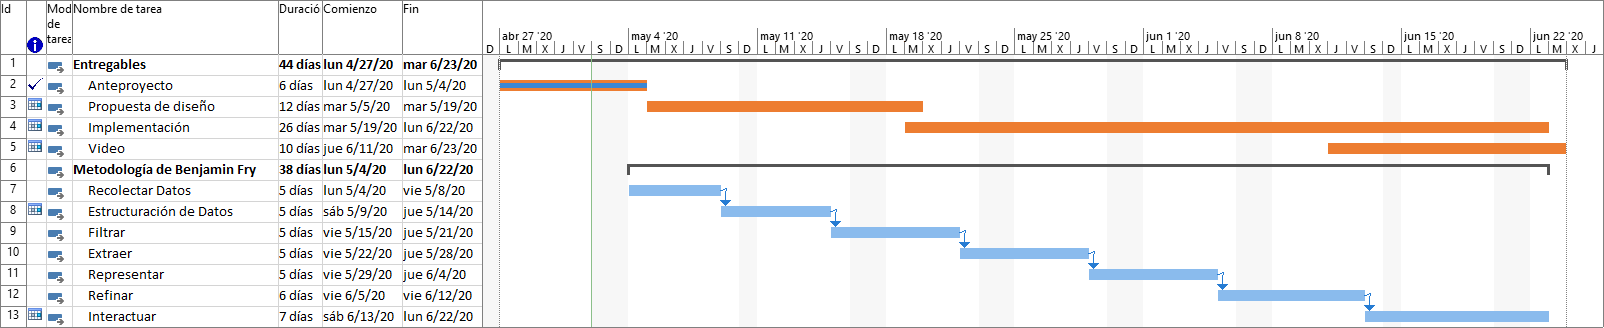
\includegraphics[width=18cm, height=14cm, keepaspectratio]{./img/cronograma_proyecto.png}
		\caption{Cronograma de trabajo }
		\label{fig:cronograma}
	\end{figure}



\bibliography{proyecto_visualizacion}{}
\bibliographystyle{acm}

\end{document}

